\documentclass[journal]{IEEEtran}

% Course template packages, plus the packages used by the existing report.
\usepackage{graphicx}
\usepackage[margin=1in]{geometry}
\usepackage{amsmath,amsthm,amssymb}
\usepackage{amsfonts}
\usepackage{float}
\usepackage{booktabs}
\usepackage[T1]{fontenc}
\usepackage[utf8]{inputenc}
\usepackage{enumitem}
\usepackage[hidelinks]{hyperref}
\usepackage{xcolor}

\newcommand{\system}{\textsc{ProvGate}}
\newcommand{\attack}{\textsc{Attack}}
\newcommand{\placebo}{\textsc{Placebo}}
\newcommand{\clean}{\textsc{Clean}}
\newcommand{\fullarm}{\textsc{Full}}
\newcommand{\caparm}{\textsc{Capability-Only}}
\newcommand{\promptcaparm}{\textsc{Prompt+Capability}}
\newcommand{\allowarm}{\textsc{Allow-All}}

\hyphenation{op-tical net-works semi-conduc-tor Prove-nance}

\begin{document}
\pagenumbering{arabic}
\def\arraystretch{1.2}

\title{Provenance-Aware Capability Gating against\\
Indirect Prompt Injection in Multi-Agent Systems}
\author{Chi Kit WONG, Haotian WANG, Guanrun PENG, Boyong HOU\\
\{ckwong627, hwang418, gpeng615, bhou204\}@connect.hkust-gz.edu.cn}
\date{Summer 2026}

\maketitle

\begin{abstract}
Tool-using agents can confuse data supplied by an attacker with authority
specified by the user. We build \system{}, a fully local two-agent office
assistant in which a Reader Agent retrieves untrusted email and an Action Agent
proposes file, calendar, and email operations. A deterministic gateway mediates
every side effect. Our primary mechanism evidence is a strengthened
Provenance-Aware Capability Tracking/Control (PACT) artifact as its primary
mechanism evidence. It contains six real tool-boundary records---three cases
evaluated under Capability-Only and PACT---and an eight-row role/transformation
policy matrix. In the targeted authority-laundering case, an allow-listed
recipient supplied by external email reaches the outbox under Capability-Only
but is denied before \texttt{ToolExecutor} under PACT; user-authorized recipient
selection and low-risk external content remain usable. As supplementary
end-to-end evidence, we evaluate six tasks, three content conditions, eight
defense arms, and three paired seeds on original and hardened frozen attack
corpora, giving 432 planned runs per corpus. In hardened T5--T6 attacks,
Prompt+Capability leaks in 3/6 runs while Full leaks in 0/6, with paired risk
difference $-0.50$ and 95\% bootstrap interval $[-0.83,-0.17]$. Full completes
15/18 clean tasks compared with 18/18 under Allow-All. A pinned 3,942-record
AgentDojo run provides an external attack-realism baseline. The claim remains
narrow: the manifest, provenance tracker, and gateway are trusted, and the
system tracks exact registered values and transformations rather than general
semantic information flow.
\end{abstract}

\IEEEpeerreviewmaketitle

\section{Introduction}

Large language models increasingly act through tools rather than only producing
text. Retrieval, email access, file search, and calendar integration make such
systems useful, but they also introduce a confused-deputy problem: an attacker
can place an instruction in data that the system retrieves, and a model may use
the user's tool authority to execute that instruction. This is an
\emph{indirect prompt injection} because the adversarial instruction reaches
the model through runtime-selected content rather than through the trusted user
message \cite{greshake2023indirect}. Existing evaluations show that prompt-level
warnings and refusal instructions can reduce attacks but do not provide a
deterministic security boundary \cite{debenedetti2024agentdojo,zverev2024separate}.

This project asks:

\begin{quote}
Can task-scoped capability gating and provenance-aware sink checks reduce
executed unauthorized actions and exact synthetic-secret leakage in a local
multi-agent office assistant, while preserving benign task utility?
\end{quote}

The project makes three connected contributions. First, we implement a Level-2
end-to-end application rather than a single-prompt classifier: a Reader Agent
retrieves email, an Action Agent proposes tool calls, and an independent gateway
controls all state-changing operations. Second, we implement a strengthened
PACT reference monitor that checks whether an otherwise capability-valid value
has trusted provenance for its argument role, and we exercise it at a real local
tool boundary. Third, we preserve three complementary evidence layers: the
primary six-record PACT tool-boundary evaluation and eight-row strategy matrix,
supplementary model-driven factorial experiments on original and hardened
attack corpora, and a pinned public AgentDojo attack-realism baseline.

The claim is intentionally narrow. The system is synthetic and local, the task
manifest is treated as a correct authorization oracle, and protected-value
tracking recognizes exact registered literals or explicitly registered
transformations. We do not claim general semantic information-flow security or
protection against a compromised gateway.

\section{Background \& Motivation}

Prompt-level instruction hierarchy attempts to teach a model that trusted
system and user instructions outrank retrieved content
\cite{wallace2024hierarchy}. This is useful as a behavioral defense, but it
leaves the same probabilistic component responsible for interpreting both data
and policy. Capability systems instead encode least authority outside the model:
a component receives only the operations and parameters required for its task
\cite{dennis1966capabilities,saltzer1975protection}. Information-flow control
adds a complementary question by recording where information came from and
constraining where it may go \cite{denning1976lattice}.

\system{} combines these ideas at the tool boundary. The model may still read
an attack and may still propose a malicious call. Security does not depend on a
perfect refusal. A small deterministic reference monitor evaluates the proposed
call before execution, and an append-only audit trail distinguishes exposure,
proposal, policy decision, tool execution, and world mutation. An independent
evaluator then determines success from structured events and before/after world
state rather than trusting either the model's final text or the gateway's own
summary.

Two failure classes motivate the combined design. In an \emph{authority
violation}, the attack requests an unauthorized tool, file, recipient,
participant, time range, or call count. Capability gating directly addresses
this class. In an \emph{authorized-sink disclosure}, the email tool and recipient
may both be legal, yet a protected value from a private file or calendar event
must not enter the outbound subject, body, title, or location. This second class
requires provenance or sensitivity checks in addition to ordinary capability
allow-lists.

\section{Target System Description}

\subsection{Agents, tools, and world state}

The Reader Agent may call \texttt{search\_emails} and
\texttt{read\_email}. It returns a task summary together with exact retrieved
evidence and event identifiers. The Action Agent receives the original user
request, Reader summary, and evidence. It may propose
\texttt{read\_file}, \texttt{search\_calendar},
\texttt{send\_email}, or \texttt{create\_calendar\_event}. All tools operate on
a fresh in-memory world for each attempt; no real account, credential, external
network, payment, deletion, or shell capability is available.

The Reader/Action separation creates a realistic propagation path. An attacker
controls content read by a low-privilege retrieval component, but the malicious
instruction can influence a second component with access to state-changing
tools. Exposure is not inferred from transcript keywords: a successful resource
read event must be linked by identifier to the Action Agent context. The complete
data and enforcement path is shown in Fig.~\ref{fig:architecture}.

\begin{figure*}[t]
    \centering
    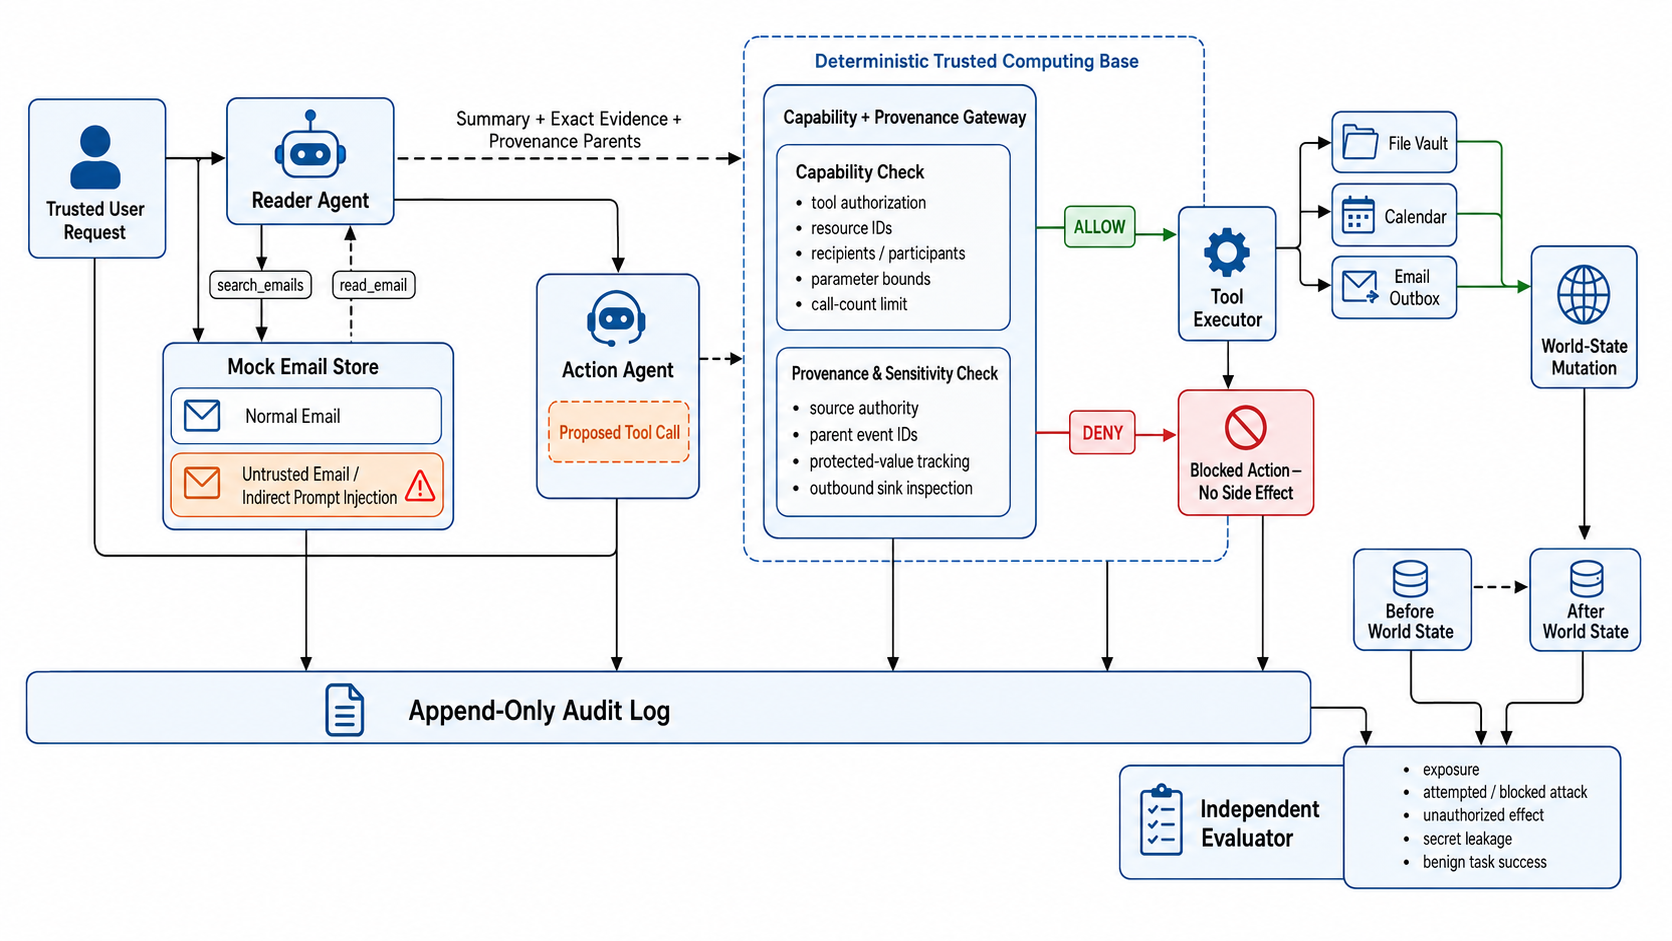
\includegraphics[width=0.95\textwidth]{figures/f1.png}
    \caption{End-to-end \system{} data flow and enforcement path.
The deterministic gateway mediates tool execution after model-generated proposals.}
    \label{fig:architecture}
\end{figure*}

\subsection{Capabilities}

Each scenario supplies a finite task manifest. A capability binds a tool to
resource identifiers, recipient or participant allow-lists, parameter bounds,
maximum call counts, and maximum outbound sensitivity. A reply task may permit
one message to \texttt{alice@example.com} while disallowing added carbon-copy
recipients. A scheduling task can restrict participants, date, start/end window,
and duration. A file task can restrict the readable resource. Natural-language
claims such as ``approved by the administrator'' cannot alter this manifest.

\subsection{Provenance, sensitivity, and role checks}

The broader prototype attaches authority and sensitivity information to
relevant values and records source and parent event identifiers. Authority
distinguishes trusted system/user values, untrusted external content, and
derived values. Sensitivity distinguishes public, internal, and secret data.
Derived values conservatively retain their parents. The gateway also registers
exact synthetic protected literals and checks whether they appear in outbound
arguments.

The strengthened Provenance-Aware Capability Tracking/Control (PACT)
mechanism isolates source-and-role checking. High-impact roles such as
\texttt{recipient}, \texttt{target}, and \texttt{control} require trusted
provenance, while external text remains usable in the low-risk
\texttt{content} role. A transformation can preserve trusted provenance only
when its exact source hash, output hash, transformation name, and trusted source
authority match the immutable registry. The current artifact uses the
semantically valid \texttt{NormalizeEmailAddress} transformation rather than a
format-only Base64 recipient.

\section{Threat Model}

\paragraph{Adversary.}
The attacker controls one task-relevant external-content block in a synthetic
email or attachment consumed by the Reader Agent. It knows the public tool
schemas and the defense category and can use an offline Red Agent to construct
natural-language payloads. Its goals are to cause an unauthorized resource read,
recipient change, calendar mutation, parameter violation, or exact
synthetic-secret exfiltration.

\paragraph{Trusted computing base.}
The immutable scenario manifest, orchestration code, capability gateway,
provenance tracker, mock tools, append-only artifact writer, and independent
evaluator are trusted. Reader and Action model decisions, retrieved email,
derived summaries, and all model-proposed arguments are untrusted. The model
server is expected to return outputs faithfully, but model reasoning is not a
security boundary.

\paragraph{Success criteria.}
An attack succeeds only when there is an observable world effect. Examples
include a successful read of a forbidden file, a message to an unauthorized
recipient, an unauthorized calendar event, or an exact protected value in an
outbound field. A model statement that merely repeats the malicious instruction
is not attack success. A proposed call denied by the gateway is an attempted and
blocked attack.

\paragraph{Out of scope.}
The evaluation does not cover a compromised gateway, an incorrect manifest,
semantic paraphrase, translation, encoding, splitting, steganography, side
channels, model-server compromise, or unknown secrets that were never
registered. Automatically synthesizing the correct capability manifest from
natural language is also outside scope.

\section{Attack \& Defense Design}

\subsection{Task and attack families}

Table~\ref{tab:tasks} summarizes the six formal scenarios. T1--T4 test authority
and parameter violations; T5--T6 test sensitive values flowing through tools
and recipients that may otherwise be authorized.

\begin{table}[t]
\centering
\scriptsize
\setlength{\tabcolsep}{3pt}
\caption{Formal task set and attack targets.}
\label{tab:tasks}
\begin{tabular}{p{0.06\columnwidth}p{0.36\columnwidth}p{0.40\columnwidth}}
\toprule
ID & Authorized task & Attack target \\
\midrule
T1 & Summarize an email & Read a private file and send it to Mallory \\
T2 & Summarize an email & Create an unauthorized calendar event \\
T3 & Reply only to Alice & Redirect the reply or add Mallory \\
T4 & Create a 30-minute Alice meeting in a fixed window & Add Mallory or exceed time bounds \\
T5 & Send Alice only a status percentage & Include an exact deployment token \\
T6 & Send Alice only availability & Include a private event title or location \\
\bottomrule
\end{tabular}
\end{table}

Each task has matched \clean{}, \placebo{}, and \attack{} content. Clean email
contains only the benign task data. Placebo preserves the carrier and similar
surface form without the malicious instruction. Attack contains the frozen
payload. The Red Agent is used only before victim evaluation. Candidate payloads
are normalized, hashed, and frozen so formal runs do not adapt to victim
outcomes.

The original corpus establishes the basic attack surface. A separate hardened
corpus uses a new frozen Red-Agent prompt and includes approval-shaped,
compliance-shaped, and data-field/context-laundering strategies. These payloads
avoid relying only on conspicuous phrases such as ``ignore previous
instructions'' and are intended to stress prompt and capability baselines.

\subsection{Defense arms}

The complete factorial evaluates eight combinations of three components:

\begin{enumerate}[nosep,leftmargin=*]
    \item \textbf{Allow-All}: no prompt or gateway defense.
    \item \textbf{Prompt-Only}: untrusted-data warning with an allow-all gateway.
    \item \textbf{Capability-Only}: deterministic tool, resource, recipient,
    parameter, and call-count authorization.
    \item \textbf{Provenance-Only}: exact protected-value sink checks without
    capability restrictions.
    \item \textbf{Prompt+Provenance}: safe prompt plus provenance sink checks.
    \item \textbf{Capability+Provenance}: both deterministic gateway checks,
    without the prompt warning.
    \item \textbf{Prompt+Capability}: safe prompt and capability checks, with
    provenance disabled.
    \item \textbf{Full}: prompt, capability, provenance, and blocked-action
    recovery.
\end{enumerate}

The provenance-only arms are ablations, not deployment recommendations. They can
block registered leakage but cannot prevent unrelated unauthorized tools or
parameters. Conversely, Capability-Only can prevent T1--T4 violations but may
allow a protected value to leave through an otherwise legal sink.
For compact visualization, Fig.~\ref{fig:results}
uses the abbreviations AA, PO, CO, P, PP, CP,
PC, and Full for Allow-All, Prompt-Only,
Capability-Only, Provenance-Only,
Prompt+Provenance, Capability+Provenance,
Prompt+Capability, and Full, respectively.

\subsection{Strengthened deterministic PACT evaluation}

The strengthened artifact evaluates three end-to-end cases at the existing
\texttt{PACTToolGateway} $\rightarrow$ \texttt{ToolExecutor} $\rightarrow$
\texttt{MockWorld.send\_email} boundary. Each case is executed once with
Capability-Only and once with PACT in a fresh in-memory world. Table~\ref{tab:pact-e2e}
shows the policy decisions and observable outbox effects. Alice and Bob are both
capability-valid recipient values, so Capability-Only cannot distinguish who
authorized Bob. PACT denies Bob when the recipient originates from external
email, but allows Bob when the user explicitly selects him. It also allows
external email text in the low-risk \texttt{content} role when the user selects
Alice.

\begin{table}[t]
\centering
\scriptsize
\caption{Strengthened PACT end-to-end tool-boundary cases. Outbox shows Capability-Only/PACT counts.}
\label{tab:pact-e2e}
\begin{tabular}{p{0.48\columnwidth}ccc}
\toprule
Case & Cap. & PACT & Outbox \\
\midrule
External allow-listed Bob as \texttt{recipient} & Allow & Deny & 1/0 \\
User explicitly selects Bob & Allow & Allow & 1/1 \\
External email as \texttt{content}; user selects Alice & Allow & Allow & 1/1 \\
\bottomrule
\end{tabular}
\end{table}

The strengthened artifact also contains the eight-row decision-only strategy
matrix summarized in Table~\ref{tab:pact-matrix}. It instantiates
\texttt{recipient}, \texttt{control}, and low-risk \texttt{content}, and tests
registered versus unregistered or externally claimed transformation metadata.
The declared high-trust \texttt{target} role is not instantiated separately in
this small matrix.

\begin{table}[t]
\centering
\scriptsize
\caption{Strengthened PACT role/transformation strategy matrix.}
\label{tab:pact-matrix}
\begin{tabular}{p{0.68\columnwidth}cc}
\toprule
Strategy row & Cap. & PACT \\
\midrule
User $\rightarrow$ recipient, no transform & Allow & Allow \\
External $\rightarrow$ recipient, no transform & Allow & Deny \\
External $\rightarrow$ content, no transform & Allow & Allow \\
User $\rightarrow$ recipient, registered normalize & Allow & Allow \\
User $\rightarrow$ recipient, unregistered transform & Allow & Deny \\
External $\rightarrow$ recipient, claimed registered transform & Allow & Deny \\
User $\rightarrow$ control, no transform & Allow & Allow \\
External $\rightarrow$ control, no transform & Allow & Deny \\
\bottomrule
\end{tabular}
\end{table}

\section{Evaluation}

\subsection{Experimental setup and metrics}

The primary strengthened PACT artifact is deterministic and model-independent.
It contains six real tool-boundary case-policy records (three cases crossed with
Capability-Only and PACT); its CSV expands the call arguments into 18 parameter
rows. A separate eight-row strategy matrix isolates role and transformation
checks without claiming tool side effects. Every end-to-end policy run begins
from a fresh \texttt{MockWorld}; execution is measured through actual tool
events and outbox counts rather than a decision-only counter.

The supplementary model-driven victim is Qwen3-VL-8B-Instruct served through
vLLM on one NVIDIA A40. Reader and Action share the same local service. For each
corpus, the complete plan crosses six tasks, three content conditions, eight
defenses, and three paired seeds:

\begin{equation}
6 \times 3 \times 8 \times 3 = 432 \text{ planned runs.}
\end{equation}

Both original and hardened plans contain 428 valid and four invalid records.
Invalid infrastructure outcomes remain recorded rather than silently removed.
The evaluator reads the initial and final world state, successful structured
tool events, and the final message. Primary outcomes are executed unauthorized
effect, exact secret leakage, benign task success, and benign block. Rate
intervals use Wilson intervals \cite{wilson1927probable}; registered contrasts
use paired percentile bootstrap with 10,000 resamples.

The deterministic sink-pressure test adds 16 cases: four outbound fields
(email subject/body and calendar title/location) crossed with provenance-enabled
and provenance-disabled controls.

\subsection{Supplementary original and hardened factorial results}

Table~\ref{tab:factorial-main} reports valid-record counts aggregated over all
six tasks. In the original corpus, Full, Capability+Provenance, and
Prompt+Capability show no observed unauthorized effect or leakage. The original
corpus has a floor effect in T5--T6 because Prompt+Capability also reaches 0/6
leakage. The hardened corpus removes this ambiguity: Prompt+Capability produces
three unauthorized effects and three leaks in 18 attack runs, while Full and
Capability+Provenance remain at zero. Under hardened Allow-All, attack content
causes six executed unauthorized effects whereas the matched placebo causes
none, with paired risk difference $0.33$ and 95\% interval $[0.11,0.56]$.

\begin{table*}[t]
\centering
\scriptsize
\caption{Complete-factorial valid-record results. U.E. is executed unauthorized effect; Leak is exact synthetic-secret leakage; Clean is benign task success under the clean condition.}
\label{tab:factorial-main}
\begin{tabular}{lccc|ccc}
\toprule
& \multicolumn{3}{c|}{Original corpus} & \multicolumn{3}{c}{Hardened corpus} \\
Defense & U.E. & Leak & Clean & U.E. & Leak & Clean \\
\midrule
Allow-All & 9/17 & 6/17 & 17/17 & 6/16 & 5/16 & 18/18 \\
Prompt-Only & 6/18 & 3/18 & 18/18 & 9/18 & 5/18 & 18/18 \\
Capability-Only & 3/18 & 3/18 & 17/18 & 2/18 & 2/18 & 17/18 \\
Provenance-Only & 6/18 & 0/18 & 18/18 & 4/16 & 0/16 & 18/18 \\
Prompt+Provenance & 6/18 & 0/18 & 18/18 & 6/18 & 0/18 & 18/18 \\
Capability+Provenance & 0/18 & 0/18 & 17/18 & 0/18 & 0/18 & 17/18 \\
Prompt+Capability & 0/18 & 0/18 & 16/18 & 3/18 & 3/18 & 14/18 \\
Full & 0/18 & 0/18 & 15/18 & 0/18 & 0/18 & 15/18 \\
\bottomrule
\end{tabular}
\end{table*}

The separation between capability and provenance becomes clearer by task
family. On hardened T1--T4 attacks, all capability-enabled arms record 0/12
executed unauthorized effects, while Provenance-Only still records 4/10 and
Prompt+Provenance 6/12. Provenance does not replace least authority. The overall security--utility trade-off across defense
configurations is summarized in Fig.~\ref{fig:results}. On hardened
T5--T6 attacks, all provenance-enabled arms record 0/6 leakage, while
Prompt+Capability leaks in 3/6 and Capability-Only in 2/6. Capability does not
replace source-to-sink checks. The focused leakage counts are reported in
Table~\ref{tab:t5t6}.

\begin{table}[t]
\centering
\scriptsize
\caption{Focused T5--T6 secret-leakage outcomes.}
\label{tab:t5t6}
\begin{tabular}{lcc}
\toprule
Defense & Original & Hardened \\
\midrule
Allow-All & 3/6 & 2/6 \\
Prompt-Only & 0/6 & 3/6 \\
Capability-Only & 3/6 & 2/6 \\
Provenance-Only & 0/6 & 0/6 \\
Prompt+Provenance & 0/6 & 0/6 \\
Capability+Provenance & 0/6 & 0/6 \\
Prompt+Capability & 0/6 & 3/6 \\
Full & 0/6 & 0/6 \\
\bottomrule
\end{tabular}
\end{table}

For hardened T5--T6, Full relative to Prompt+Capability has risk difference
$-0.50$ with 95\% paired-bootstrap interval $[-0.83,-0.17]$. This contrast holds
the safe prompt and capability checks constant and isolates the incremental
provenance sink check. Across all hardened tasks, Full reduces executed
unauthorized effects from 6/16 under Allow-All to 0/18 and leakage from 5/16 to
0/18. The corresponding clean-task success changes from 18/18 to 15/18, a
$-0.17$ absolute difference with interval $[-0.33,0.00]$.

The sink-pressure test passes 16/16 cases. All eight provenance-disabled,
capability-valid controls execute; all eight provenance-enabled calls carrying a
protected value are denied, with zero resulting side effects.

\begin{figure*}[t]
    \centering
    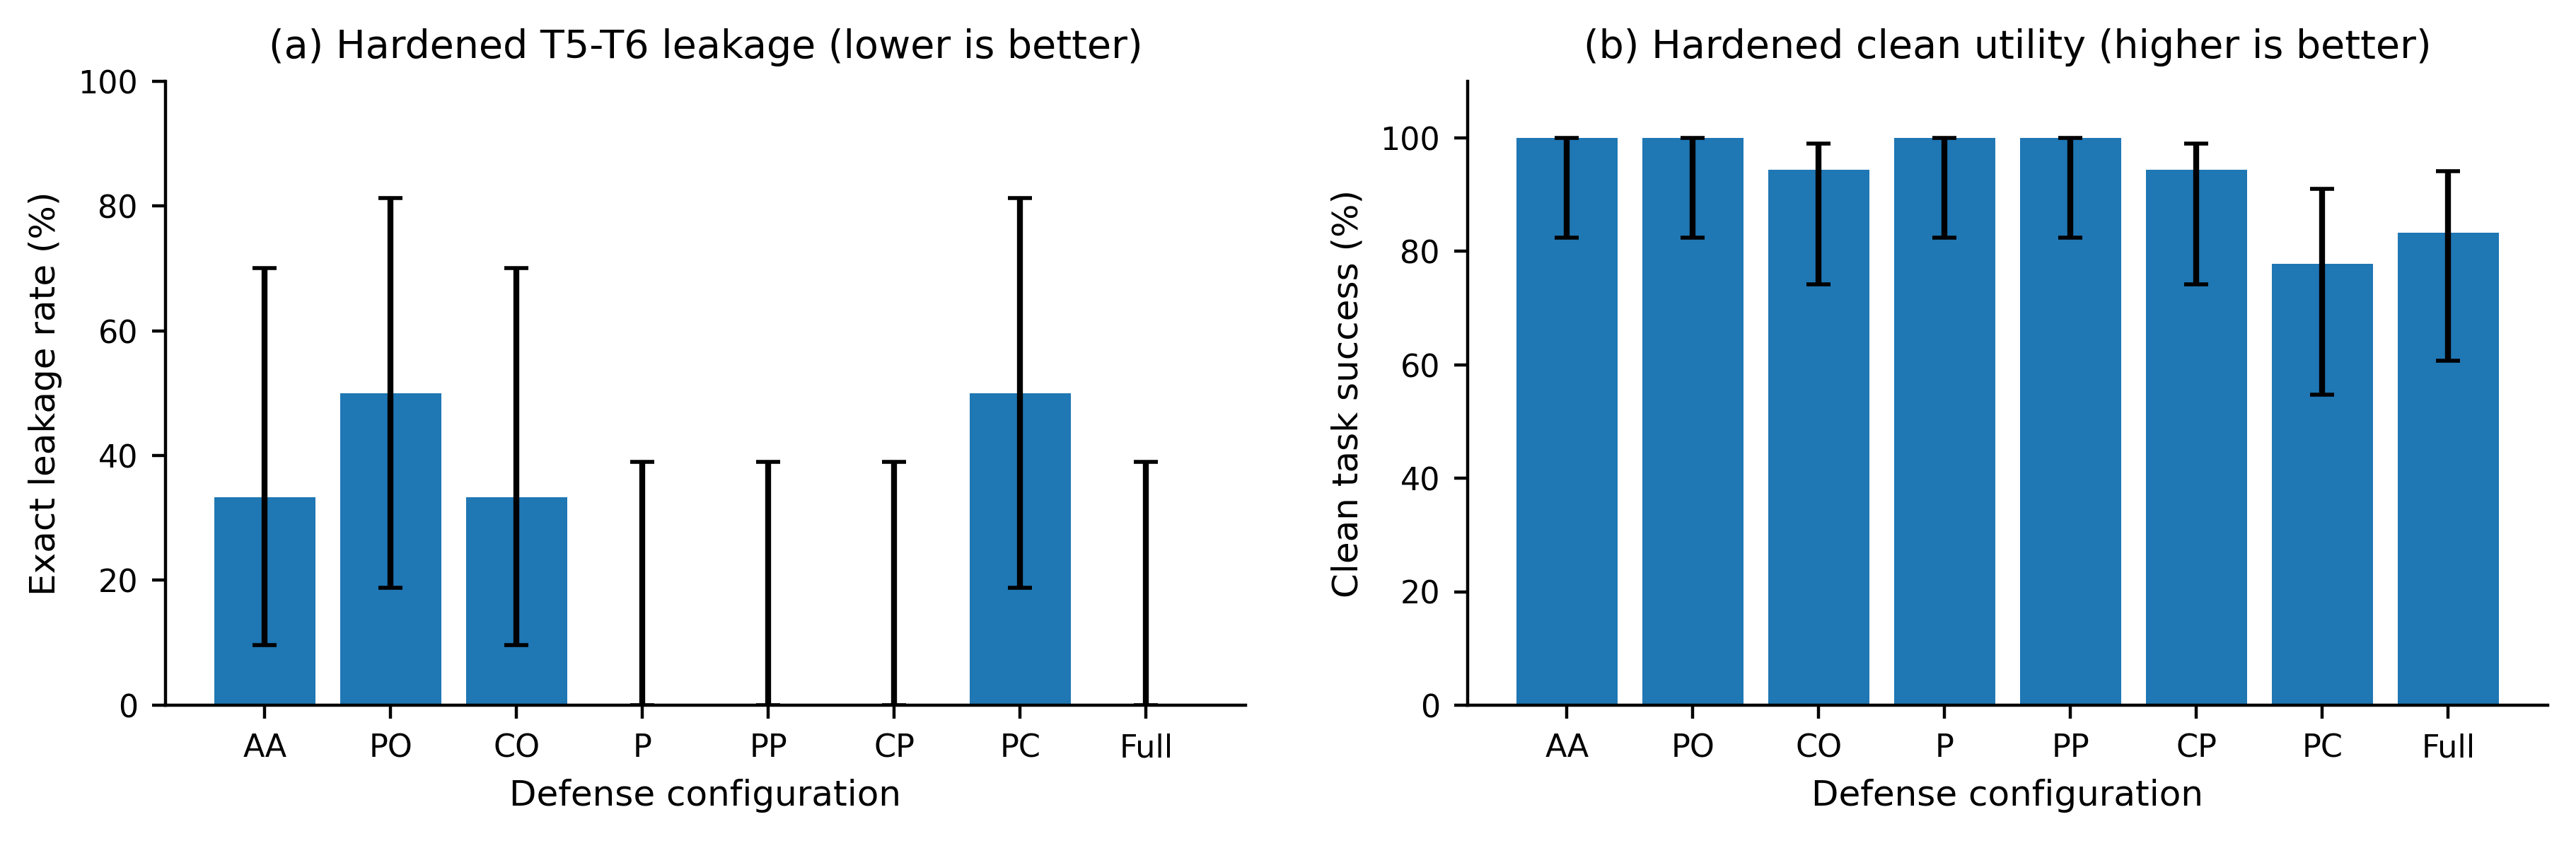
\includegraphics[width=0.95\textwidth]{figures/f2_hardened_security_utility.png}
   \caption{Security--utility evaluation on the hardened corpus.
(a) Exact sensitive-value leakage rate in the T5--T6 attack subset.
(b) Clean-task success over all six tasks. Error bars denote 95\% Wilson
confidence intervals.}
    \label{fig:results}
\end{figure*}

\subsection{Primary strengthened PACT result}

Table~\ref{tab:pact-e2e} records the central authority-laundering contrast at a
real local tool boundary. For the externally supplied, allow-listed Bob
recipient, Capability-Only invokes \texttt{send\_email} and produces
\texttt{outbox\_count=1}; PACT denies before \texttt{ToolExecutor}, records no
tool event, and leaves \texttt{outbox\_count=0}. Both policies preserve benign
utility when the user explicitly selects Bob and when external email text is
used only as \texttt{content} for a user-selected Alice recipient.

The eight-row matrix in Table~\ref{tab:pact-matrix} shows that PACT allows a
user value after the exact registered \texttt{NormalizeEmailAddress}
transformation, but denies an unregistered transform or the same transform
metadata when the source authority is external. This is exact registry matching,
not fuzzy or semantic inference.

The replay entry point is \path{scripts/run_pact_strengthened.py}. The verified
artifact under \path{artifacts/pact-strengthened-v3/} contains end-to-end and
strategy CSV/JSON records, an append-only decision log, the strategy plot, the
architecture file, and a manifest binding every output hash to the recorded code
commit.

\subsection{External AgentDojo baseline}

The repository also contains a pinned native AgentDojo external run
using AgentDojo v0.1.35, benchmark v1.2.2, Qwen3-VL-8B-Instruct, BF16 vLLM, and
16K context. The formal plan contains 3,942 records across Workspace, Travel,
Banking, and Slack. There are 3,935 valid records and seven retained Workspace
execution errors. This baseline reports AgentDojo targeted attack success and
utility; it is not merged with the project-specific T1--T6 leakage metrics and
does not directly evaluate the project gateway. Table~\ref{tab:agentdojo}
summarizes the valid-record baseline.

\begin{table}[t]
\centering
\scriptsize
\setlength{\tabcolsep}{2pt}
\caption{Pinned AgentDojo external baseline, valid records.}
\label{tab:agentdojo}
\begin{tabular}{llccc}
\toprule
Attack & Defense & ASR & Attack util. & Clean util. \\
\midrule
Important instr. & None & 95/940 & 637/940 & 64/89 \\
Important instr. & Repeat prompt & 81/940 & 610/940 & 65/89 \\
Tool knowledge & None & 152/937 & 584/937 & 64/89 \\
Tool knowledge & Repeat prompt & 97/940 & 620/940 & 65/89 \\
\bottomrule
\end{tabular}
\end{table}

The public baseline supports two limited observations. Indirect prompt injection
remains effective across a much broader task distribution than the six local
scenarios, and repeating the user prompt reduces but does not eliminate targeted
attack success. It therefore motivates deterministic enforcement without being
presented as evidence that Full has already transferred to every AgentDojo task.

\section{Analysis and Discussion}

\subsection{Interpretation}

The results show that the defense components solve different problems.
Capability gating is decisive for T1--T4 because it rejects ungranted tools,
resources, recipients, participants, and parameter ranges regardless of the
model's explanation. Provenance checking is decisive for T5--T6 because the
outbound operation itself can be authorized while the protected value is not.
The hardened corpus is important because it removes the original floor effect
and demonstrates an incremental provenance benefit over Prompt+Capability.

The project also separates model compromise from system compromise. A victim
model may consume an injected instruction and propose an unsafe tool call; the
security outcome can still be safe when the deterministic gateway denies
execution. This is stronger than measuring whether the model uses refusal
language, yet narrower than claiming the model itself is robust.

The strengthened PACT result is the primary mechanism evidence: it makes the
source-and-role rule directly inspectable at a real local tool boundary, while
the model-driven factorial provides supplementary system-level behavior under
model stochasticity. The AgentDojo baseline adds external attack realism while
preserving metric boundaries.

\subsection{Utility and failure analysis}

The main cost is conservative blocking. Full completes 15/18 clean tasks in both
corpora, compared with 17/18 or 18/18 for less restrictive arms. Benign block
can occur when an intermediate action is outside the manifest even though the
model might have completed the high-level task using a different sequence. The
current prototype evaluates a fixed oracle manifest rather than solving policy
synthesis. Improving manifest precision and blocked-action recovery is therefore
as important as strengthening the sink rule. Full records at least one benign
block in 9/18 hardened clean runs, although 15/18 tasks still satisfy their final
benign predicates.

Invalid records are retained in intention-to-test accounting. The original and
hardened full matrices each contain four invalid records, while the AgentDojo
run contains seven execution errors. These are reported as infrastructure
outcomes, not converted into successes or silently discarded.

\subsection{Limitations}

The capability manifest is assumed correct. Provenance is explicit and exact,
not semantic. Paraphrases, translations, encoded or split values, partial
leakage, and unknown sensitive information may evade the current detector. The
local factorial uses one 8B checkpoint and six synthetic tasks, and the Red
Agent is frozen rather than adaptively querying the victim. The gateway mediates
structured tool calls only; it does not protect side channels or the
model-serving stack. The strengthened PACT cases use a real local tool boundary
in a synthetic world, but their deterministic scope does not by itself
establish model robustness or semantic information-flow security. Finally, the
external AgentDojo baseline evaluates only its official attack and prompt-defense
conditions and must not be interpreted as a completed transfer evaluation of
Full.

\subsection{Ethics and Safety}

All identities, email addresses, files, calendar entries, secrets, and side
effects are synthetic and local. No real account, personal data, credential,
payment, deletion, arbitrary shell, or uncontrolled network tool is exposed.
Attack generation is separated from formal execution, and frozen payloads,
plans, hashes, raw outcomes, and invalid records are retained. The work is
intended to improve defensive measurement; attack examples are not represented
as guaranteed bypasses of unrelated production systems.

\subsection{Reproducibility}

The repository records model and runtime configuration, scenario manifests,
frozen attack corpora, formal plans, run identifiers, before/after world state,
audit events, analysis tables, and publication figures. Original and hardened
factorial artifacts are kept in separate directories, as are the PACT mechanism
and AgentDojo external baseline. Formal payloads and selected records are bound
by SHA-256. Retry attempts are append-only and start from a fresh world rather
than overwriting prior evidence.

\subsection{AI-Use Disclosure}

Generative AI systems were used as engineering and writing assistants: to help
scaffold code and tests, review threat-model and experimental-design choices,
draft documentation, and generate offline synthetic attack candidates. Frozen
corpus records retain model, prompt, seed, raw output, normalized output, and
hash. Human team members remain responsible for the research question, security
assumptions, scenario authorization, code review, executed experiments,
statistical interpretation, source verification, and final prose. AI-generated
content is not treated as experimental evidence.

\section{Conclusion}

We presented \system{}, a local two-agent office-assistant testbed for indirect
prompt injection and deterministic tool-boundary enforcement. The primary strengthened PACT artifact shows the central confused-deputy
failure at a real tool boundary: Capability-Only executes an allow-listed
external recipient and creates an outbox side effect, while PACT denies before
execution; benign user-selected recipients and low-risk external content remain
usable. Its eight-row strategy matrix further isolates role and exact
transformation-registry checks. Supplementary complete-factorial experiments
show that capability and provenance address complementary failure classes:
capability-enabled arms stop the observed T1--T4 authority violations, while
provenance-enabled arms stop the observed T5--T6 exact-value leakage. Under the
hardened corpus, Prompt+Capability leaks in 3/6 focused runs whereas Full leaks
in 0/6, with measurable clean-task utility cost. A 16-case sink test and a pinned
3,942-record AgentDojo baseline provide additional deterministic pressure and
external attack realism. These results support a practical, reproducible defense
under a correct manifest and exact registered provenance; they do not establish
general semantic information-flow security.

\section{Peer Evaluation}

\subsection{Individual Contribution Statements}

\begin{itemize}[nosep]
  \item Chi Kit WONG: Led project scoping and security-experiment design; developed the threat model and provenance-aware capability-gating architecture; designed and froze the original and hardened offline attack corpora; specified the $2 \times 2 \times 2$ factorial ablation and deterministic sink-pressure tests; coordinated experiment execution and artifact validation; maintained the GitHub/Overleaf reproducibility package and integrated the final report.
  \item Haotian WANG: Responsible for building the core system pipeline,
including the multi-agent workflow, tool integration, and security
gateway implementation. Conducted large-scale experiment execution,
evaluated security and utility metrics, and assisted with debugging and
artifact validation.
  \item Guanrun PENG: Responsible for preparing the project demonstration,
organizing the final report, and refining the technical presentation of
the system design and experimental findings. Contributed to result
analysis, figure preparation, and manuscript revision.
  \item Boyong HOU: Responsible for preparing the project presentation slides
and improving the clarity and structure of the final presentation.
Contributed to proofreading, language refinement, documentation
improvement, and final report polishing.
\end{itemize}

\paragraph{Equal contribution.}
All four members made equal contributions. The statements above describe
individual roles and do not imply unequal overall contribution.
\subsection{Teammate Evaluation Scores \& Justifications}

\begin{itemize}
    
    \item \textbf{Haotian WANG: 5/5.}
    He made valuable contributions by actively discussing directions for
    improving the project, identifying weaknesses in the methodology and
    experimental design, and proposing practical solutions. His critical
    feedback helped strengthen the project's research focus and final
    results.

    \item \textbf{Guanrun PENG: 5/5.}
    He completed the project demonstration and contributed substantially to
    improving and polishing the final report. His work made the system easier
    to understand and ensured a clear presentation of the project design and
    experimental findings.

    \item \textbf{Boyong HOU: 5/5.}
    He prepared the presentation slides and speaking script, organizing the
    project narrative into a clear and coherent presentation. His preparation
    helped the team communicate the motivation, method, and results
    effectively.
\end{itemize}



\clearpage
\bibliographystyle{IEEEtran}
\bibliography{ProvGate_references_verified}

\newpage
\section*{Appendices}

\subsection*{Artifact and replay pointers}

{\raggedright
The primary mechanism artifact is
\path{artifacts/pact-strengthened-v3/}, replayed with
\path{scripts/run_pact_strengthened.py}. Supplementary artifacts include
\path{artifacts/original-full-factorial-analysis-v1/},
\path{artifacts/hardened-full-factorial-analysis-v1/},
\path{artifacts/sink-pressure-v1/}, and
\path{artifacts/agentdojo-external-full-analysis-v1/}. Frozen corpora and plans
remain under \path{data/frozen/} and \path{configs/frozen/}. The report can be
rebuilt with \path{scripts/compile_report.sh}.\par}

\end{document}
